%\documentclass[a4paper,11pt]{amsart}
\documentclass[a4paper,UKenglish,cleveref,autoref]{lipics-v2021}
%This is a template for producing LIPIcs articles. 
%See lipics-manual.pdf for further information.
%for A4 paper format use option "a4paper", for US-letter use option "letterpaper"
%for british hyphenation rules use option "UKenglish", for american hyphenation rules use option "USenglish"
%for section-numbered lemmas etc., use "numberwithinsect"
%for enabling cleveref support, use "cleveref"
%for enabling cleveref support, use "autoref"
 

%\graphicspath{{./graphics/}}%helpful if your graphic files are in another directory

\bibliographystyle{plainurl}% the mandatory bibstyle

\title{Max Independent Set Remains NP-hard when Excluding a Planar Induced Minor}
\titlerunning{MIS Remains NP-hard when Excluding a Planar Induced Minor}

%\author{ }{ }{}{}{}
%\authorrunning{ }
%\Copyright{ }

\author{\'{E}douard Bonnet}{CNRS, ENS de Lyon, Université Claude Bernard Lyon 1, LIP UMR 5668, Lyon, France \and \url{http://perso.ens-lyon.fr/edouard.bonnet}}{edouard.bonnet@ens-lyon.fr}{https://orcid.org/0000-0002-1653-5822}{}
\author{Yeonsu Chang}{Department of Mathematics, Hanyang University, Seoul, South Korea \and \url{yeonsuchang.com}}{yeonsu@hanyang.ac.kr}{}{}

%mandatory, please use full name; only 1 author per \author macro; first two parameters are mandatory, other parameters can be empty.

\authorrunning{\'E. Bonnet and Y. Chang}

\Copyright{Édouard Bonnet, Yeonsu Chang}%TODO mandatory, please use full first names. LIPIcs license is "CC-BY";  http://creativecommons.org/licenses/by/3.0/

%\ccsdesc[100]{Theory of computation → Graph algorithms analysis}
%\ccsdesc[100]{Theory of computation → Fixed parameter tractability}%TODO mandatory: Please choose ACM 2012 classifications from https://dl.acm.org/ccs/ccs_flat.cfm 

%\keywords{Twin-width, lower bounds}%TODO mandatory; please add comma-separated list of keywords

\category{}%optional, e.g. invited paper

\relatedversion{}%optional, e.g. full version hosted on arXiv, HAL, or other respository/website
%\relatedversion{A full version of the paper is available at \url{...}.}

\supplement{}%optional, e.g. related research data, source code, ... hosted on a repository like zenodo, figshare, GitHub, ...

%\funding{(Optional) general funding statement \dots}%optional, to capture a funding statement, which applies to all authors. Please enter author specific funding statements as fifth argument of the \author macro.

%\acknowledgements{We thank Théo Pierron and Jean-Florent Raymond with whom this project started. We also thank Tuukka Korhonen, Daniel Lokshtanov, and Martin Milanič for some discussions, and in particular for asking about the flow problem (as opposed to the linkage one).}%optional

\nolinenumbers %uncomment to disable line numbering

\hideLIPIcs  %uncomment to remove references to LIPIcs series (logo, DOI, ...), e.g. when preparing a pre-final version to be uploaded to arXiv or another public repository

%Editor-only macros:: begin (do not touch as author)%%%%%%%%%%%%%%%%%%%%%%%%%%%%%%%%%%
\EventEditors{John Q. Open and Joan R. Access}
\EventNoEds{2}
\EventLongTitle{42nd Conference on Very Important Topics (CVIT 2016)}
\EventShortTitle{CVIT 2016}
\EventAcronym{CVIT}
\EventYear{2016}
\EventDate{December 24--27, 2016}
\EventLocation{Little Whinging, United Kingdom}
\EventLogo{}
\SeriesVolume{42}
\ArticleNo{23}

%%%%%%%%%%%%%%%%%%%%%%%%%%%%

\usepackage[utf8]{inputenc}  

%Default font encoding doesn't support Polish characters
\usepackage[T1]{fontenc}
\usepackage{lmodern}

\usepackage{amsmath}  
\usepackage{amssymb}
\usepackage{amsthm}
\usepackage{bbm}
\usepackage{accents}
\usepackage{complexity}

\usepackage{booktabs}
\usepackage{paralist}
%\usepackage{bm}
%\usepackage{hyperref}
%\usepackage{mathrsfs}
%\usepackage{mathtools} 
%\usepackage{phdalgo}
\usepackage{fixmath}
%\usepackage{fullpage}
%\usepackage{interval}
%\usepackage{kbordermatrix}
%\usepackage[capitalize]{cleveref}


\makeatletter
\newtheorem*{rep@theorem}{\rep@title}
\newcommand{\newreptheorem}[2]{%
\newenvironment{rep#1}[1]{%
 \def\rep@title{#2 \ref{##1}}%
 \begin{rep@theorem}}%
 {\end{rep@theorem}}}
\makeatother

\newcommand{\cmso}{\textsf{CMSO}\xspace}
\newcommand{\cmsoo}{\textsf{CMSO$_1$}\xspace}
\newcommand{\cmsot}{\textsf{CMSO$_2$}\xspace}
\newcommand{\msot}{\textsf{MSO$_2$}\xspace}

\newreptheorem{theorem}{Theorem}
\newreptheorem{lemma}{Lemma}
\newreptheorem{corollary}{Corollary}

\usepackage{pgfplots}
\usepackage{xspace}
\usepackage{tikz}
\usepackage{tikz-3dplot}

\usepackage[ruled,vlined,linesnumbered]{algorithm2e}

\usetikzlibrary{fit} 
\usetikzlibrary{arrows}
\usetikzlibrary{patterns}
\usetikzlibrary{calc}
\usetikzlibrary{shapes}
\usetikzlibrary{positioning}
\usetikzlibrary{math}
\usetikzlibrary{shapes.symbols, shapes.geometric}
\usetikzlibrary{decorations.pathreplacing,calligraphy}
\usetikzlibrary{decorations.pathmorphing, backgrounds}
\usepackage[scr=boondox,scrscaled=1.05]{mathalfa}

\newcommand{\mis}{\textsc{Max Independent Set}\xspace}
\newcommand{\smis}{\textsc{MIS}\xspace}
\newcommand{\vc}{\textsc{Vertex Cover}\xspace}
\newcommand{\vcp}{\mathsf{vc}\xspace}
\newcommand{\wei}{\mathfrak{w}}
\newcommand{\maxcut}{\mathsf{MaxCut}}

\renewcommand{\geq}{\geqslant}
\renewcommand{\leq}{\leqslant}
\renewcommand{\preceq}{\preccurlyeq}
\renewcommand{\succeq}{\succcurlyeq}
\renewcommand{\le}{\leq}
\renewcommand{\ge}{\geq}

\crefname{conjecture}{Conjecture}{Conjectures}

\newcommand{\defparproblem}[4]{
 \vspace{1mm}
\noindent\fbox{
 \begin{minipage}{0.96\textwidth}
 \begin{tabular*}{\textwidth}{@{\extracolsep{\fill}}lr} #1 & {\bf{Parameter:}} #3 \\ \end{tabular*}
 {\bf{Input:}} #2 \\
 {\bf{Question:}} #4
 \end{minipage}
 }
 \vspace{1mm}
}

\newcommand{\arxiv}[1]{\href{http://arxiv.org/abs/#1}{arXiv:#1}}

%\DeclareMathOperator{\sign}{\mathsf{sign}}
\newcommand{\card}[1]{|{#1}|}

\DeclareMathOperator*{\bigland}{\bigwedge}
\DeclareMathOperator*{\biglor}{\bigvee}

\newcommand{\Oh}{\mathcal{O}}

\newtheorem{question}{Question}%\newtheorem{lemma}[theorem]{Lemma}

\newenvironment{proofofclaim}{\noindent \textsc{Proof of the Claim:}}{\unskip\nobreak\hfill$\Diamond$\medskip}
  
\newcommand\subd[1]{#1\text{-subd}}
\newcommand\tw{\text{tw}}
\newcommand\tww{\text{tww}}

\newenvironment{edouard}[1]{\textcolor{blue}{Édouard:~#1}}{}

\begin{document}

\maketitle

\begin{abstract}
  We show that there is a fixed planar graph $H$, namely the $5 \times 5$ grid, such that \textsc{Max Independent Set} remains NP-hard in $H$-induced-minor-free graphs.
  This refutes the Dallard--Milanič--Štorgel conjecture and a weakening of it by Gartland and Lokshtanov, and by Korhonen.
\end{abstract}

\section{Introduction}\label{sec:intro}

Graph classes excluding a~planar minor have bounded treewidth~\cite{RobertsonS86}.
Thus, in them, any problem definable in \msot logic (or its optimization variants) can be solved in polynomial time~\cite{Courcelle90}.
This cannot hold in classes excluding a~planar \emph{induced} minor (where induced minors are obtained by removing vertices and contracting edges).
Indeed, a~problem like \textsc{Dominating Set} is NP-complete on graphs excluding a~5-vertex path as an induced minor~\cite{Bertossi84} (or, equivalently, as an induced subgraph).

However, no similar direct argument dismisses that possibility for the \mis problem (\smis for short).
This led Dallard, Milanič, and Štorgel to ask whether a~polynomial-time algorithm exists for \smis on any planar-induced-minor-free class.

\begin{conjecture}[Dallard--Milanič--Štorgel~\cite{DallardMS24a}]\label{conj:dms}
For every planar graph $H$, \mis can be solved in polynomial time on graphs excluding $H$ as an induced minor.
\end{conjecture}

This question, turned into a~conjecture, has garnered a~large amount of related work in the past five years.
(Let $K_t$ denote the $t$-vertex clique, $K_{s,t}$ the biclique with $s$ vertices against $t$ vertices, $P_t$ the $t$-vertex path, $C_t$ the $t$-vertex cycle, and $W_t$ the wheel obtained from $C_t$ by adding a~universal vertex.)
\Cref{conj:dms} was shown when $H$ is $K_5$ minus an edge, $K_{2,t}$, $W_4$~\cite{DallardMS24a}, $P_6$~\cite{Grzesik22}, or any windmill graph (a~matching plus a~universal vertex)~\cite{BonnetDGTW26}.

A~natural relaxation of~\cref{conj:dms} to quasipolynomial time has seen further development.

\begin{conjecture}[Gartland--Lokshtanov, Korhonen~\cite{Korhonen23}, {\cite[Question 2]{BonnetDGTW26}}]\label{conj:qdms}
For every planar graph~$H$, \mis can be solved in quasipolynomial time on graphs excluding $H$ as an induced minor.
\end{conjecture}

While \cref{conj:dms} is already open when $H = P_7$, \cref{conj:qdms} is known when $H$ is any path, any cycle~\cite{Gartland21}, a~disjoint union of triangles~\cite{BonamyBDEGHTW24}, or even~$tC_3~\uplus~C_4$~\cite{BonnetDGTW26}.

Korhonen and Lokshtanov have obtained a~subexponential algorithm, as a~byproduct of balanced separators of size $\Oh(\sqrt m)$, where $m$ is the number of edges.

\begin{theorem}[{\cite[Corollary 1.2]{KorhonenL23}}]
  For every planar graph $H$, \mis can be solved in $2^{\Tilde{\Oh}_H(n^{2/3})}$ time on $n$-vertex graphs excluding $H$ as an induced minor.
\end{theorem}

Gartland and Lokshtanov have proposed strengthenings of~\cref{conj:dms,conj:qdms} for a~family of problems.
Fix a~positive integer $t$, a~\cmsot sentence $\varphi$, i.e., a~closed formula with universal and existential quantifications over vertices, vertex subsets, and edge subsets, and counting predicates modulo some fixed integers.
The $(\tw \leqslant t,\varphi)$-\textsc{Weighted Maximum Induced Subgraph} ($(\tw \leqslant t,\varphi)$-\textsc{WMIS}) takes as input a~vertex-weighted graph $(G,w)$ and asks one either to find a~set $S \subseteq V(G)$ such that
\begin{compactitem}
\item $G[S]$ satisfies $\varphi$,
\item the treewidth of $G[S]$ is at~most $t$, and
\item the sum of weights of vertices in~$S$ is maximized subject to the above conditions,
\end{compactitem}
or to conclude that no such set $S$ exists.

Special cases of the $(\tw \leqslant t,\varphi)$-\textsc{WMIS} problem include, for instance, \smis, \textsc{Feedback Vertex Set}, and \textsc{Even Cycle Transversal}.
It was conjectured that \cref{conj:dms} more generally holds for $(\tw \leqslant t,\varphi)$-\textsc{WMIS}.

\begin{conjecture}[{\cite[Conjecture 1.4.2]{Gartland23}}]\label{conj:gl}
  For every planar graph $H$, positive integer $t$, and \cmsot sentence $\varphi$, $(\tw \leqslant t,\varphi)$-\textsc{Weighted Maximum Induced Subgraph} can be solved in polynomial time on $H$-induced-minor-free graphs.
\end{conjecture}

\subparagraph*{Our contributions.}
We refute \cref{conj:dms,conj:qdms,conj:gl} (unless P $=$ NP for \cref{conj:dms,conj:gl}, and unless NP $\subseteq$ QP for \cref{conj:qdms}) by showing the following.

\begin{theorem}\label{thm:main}
\leavevmode
% lax begin Lax222097.IndependentSetHardness
\smis is NP-hard in graphs excluding the $5 \times 5$ grid as an induced minor.
% lax end Lax222097.IndependentSetHardness
\end{theorem}

The proof is a~remarkably simple reduction from \textsc{Max Cut} on general graphs~$F$.

Look at \cref{fig:intermediate-graph}: this intermediate graph $G$ has the strong product of a~path with an edge (i.e., a~ladder with diagonals) for each \emph{row} (with each path occupying one of two sides), and a~biclique between the two sides in each column.
It is easy to show that a~cycle in~$G$ contains two vertices in the same column and on opposite sides (mentally remove all the column bicliques and consider the possible neighbors of a~leftmost vertex of the cycle).
The joint neighborhood of two such vertices contains the entire biclique and thus separates the left-hand side from the right-hand side.
Therefore, every graph with three vertex-disjoint nonadjacent cycles and a~path between every pair of cycles avoiding the neighborhood of the third cycle cannot be an induced minor of~$G$ (the $5 \times 5$ grid has this property; see~\cref{fig:grid-three-cycles}).
Indeed, consider the cycle whose neighborhood contains the biclique in between the bicliques of the other two cycles.

We then pick an appropriate induced subgraph $G_F$ of~$G$, where every odd-index column represents a~vertex of~$F$, and every edge of~$F$ ``occupies'' two rows.
From the rows of edge $e=uv \in E(F)$, we only keep the vertices in columns between that of~$u$ and that of~$v$, with the exception of four vertices; see~\cref{fig:edge-gadget}.
This defines the graph $G_F$.
Any independent set $I$ in~$G_F$ defines a~bipartition of~$V(F)$ where the part of $v \in V(F)$ depends on the side of the column of~$v$ that intersects~$I$.
This is well-defined due to the column bicliques.
Finally, the encoding of $e \in E(F)$ is such that one more vertex can be inserted in the independent set exactly when its endpoints are in distinct parts of the bipartition of~$V(F)$; see~\cref{fig:alpha-lower-bound}.

If we reduce from \textsc{Max Cut} on subcubic graphs~$F$, the previous reduction produces graphs with $\Oh(|V(F)|^2)$ vertices.
Classic reductions thus imply the following, under the Exponential-Time Hypothesis (ETH), i.e., the assumption that there is a~$\lambda > 1$ such that $n$-variable \textsc{3-SAT} cannot be solved in time $\Oh(\lambda^n)$~\cite{Impagliazzo01}. 

\begin{corollary}\label{thm:eth}
Unless the ETH fails, \mis requires time $2^{\Omega(\sqrt{n})}$ in $n$-vertex graphs excluding the $5 \times 5$ grid as an induced minor.
\end{corollary}

\subparagraph*{Future work.}
Now, \cref{conj:dms,conj:qdms} can be turned into dichotomy questions.

\begin{question}\label{q:dichotomy}
  Which planar graphs $H$ are such that \mis can be solved in (quasi)polynomial time on graphs excluding $H$ as an induced minor?
\end{question}

In fact, we give a~negative answer to~\cref{q:dichotomy} for a~graph simpler than the $5 \times 5$ grid: the cycle $C_9$ (with $V(C_9)=\{1, \ldots, 9\}$) with three additional vertices respectively adjacent to 1~and 2, 4 and 5, and 7 and 8.

One can also turn to approximation schemes.
The following conjecture is not refuted by the present work.

\begin{conjecture}\label{conj:qptas}
  For every planar graph~$H$, \mis admits a~quasipolynomial-time approximation scheme (QPTAS) on graphs excluding $H$ as an induced minor.
\end{conjecture}

\Cref{conj:qptas} is actually known to be implied by a~structural conjecture of~Gartland and Lokshtanov.

\begin{conjecture}[Gartland--Lokshtanov~\cite{Gartland23}]\label{conj:struct-gl}
For every planar graph $H$, there is a~constant $k := k(H)$ such that every $n$-vertex $H$-induced-minor-free graph $G$ admits a~set $X \subseteq V(G)$ of size at~most~$k$ such that the closed neighborhood of~$X$ is a~balanced separator of $G$.
\end{conjecture}

A~more adventurous (but still open) conjecture is the strengthening of~\cref{conj:qptas} to a~polynomial-time approximation scheme (PTAS).

\section{Hardness of MIS in Planar-Induced-Minor-Free Classes}

For any two integers $i, j$, we use $[i,j]$ as a~shorthand for $\{i, i+1, \ldots, j-1, j\}$, and $[i] := [1,i]$.
We use the standard graph-theoretic notation.
For any graph $G$, $V(G)$ and $E(G)$ denote the vertex set and edge set, respectively, of~$G$.
If $S \subseteq V(G)$, then $G[S]$ denotes the subgraph of~$G$ induced by~$S$.

\leavevmode
% lax begin Lax222097.MaxCut
We denote by $\alpha(G)$ the \emph{independence number} of~$G$, that is, the size of a~largest subset of vertices of~$G$ that are pairwise nonadjacent.
We write $\maxcut(G)$ for the number of edges in a~maximum-cardinality cut of~$G$.
% lax end Lax222097.MaxCut

\begin{reptheorem}{thm:main}
\leavevmode
% lax begin Lax222097.IndependentSetHardness
\smis is NP-hard in graphs excluding the $5 \times 5$ grid as an induced minor.
% lax end Lax222097.IndependentSetHardness
\end{reptheorem}

\begin{proof}
\leavevmode
% lax begin Lax222097Proofs.independentSet_inducedGrid_hardness
We reduce \textsc{Max Cut} in general graphs to \mis in graphs excluding a~fixed planar induced minor.
  Let $F$ be any $n$-vertex $m$-edge \textsc{Max Cut} instance.
\leavevmode
% lax begin Lax222097.ColumnGraph
We first build an intermediate graph~$G$ with vertex set
  \[ \{(i,j,s) \mid i \in [2m],~j \in [2n-1],~s \in \{0,1\}\},\]
  where we see $i$ as the row index, $j$ as the column index, and $s$ as the side, and edge set
  \[ \{(i,j,0)(i',j,1) \mid i, i' \in [2m],~j \in [2n-1]\}~\cup \]
  \[ \{(i,j,s)(i,j',s') \mid i \in [2m],~j, j' \in [2n-1], |j-j'|=1,~s, s' \in \{0,1\}\};\]
  see~\cref{fig:intermediate-graph}.

  We arbitrarily order the vertices of~$F$: $v_1, v_2, \ldots, v_n$.
  We set $C_j := \{(i,j,s) \mid i \in [2m],~s \in \{0,1\}\}$ to be the \emph{$j$th column}.
  We see $C_{2j-1}$ as the column of~$v_j$, for every $j \in [n]$.
  The columns of even index do \emph{not} represent a~vertex of~$F$.
  Similarly, a~\emph{row} is any set $\{(i,j,s) \mid j \in [2n-1],~s \in \{0,1\}\}$ with $i \in [2m]$.
  We reserve two rows for each edge $e \in E(F)$, and denote them by $R'_{e,0}$ and $R'_{e,1}$.
  For convenience, we denote by $e^0, e^1 \in [2m]$ the row indices of $R'_{e,0}, R'_{e,1}$, respectively. 
% lax end Lax222097.ColumnGraph

\begin{figure}[!ht]
\centering
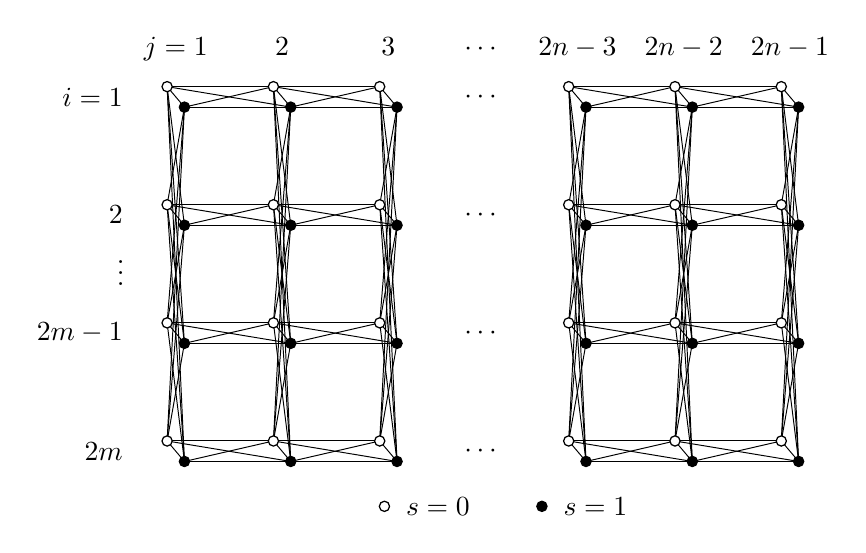
\begin{tikzpicture}[
  edge/.style={draw=black, line width=.35pt, line cap=round},
  vertex/.style={circle, draw=black, line width=.45pt, minimum size=3.7pt, inner sep=0pt},
  side 0/.style={vertex, fill=white},
  side 1/.style={vertex, fill=black}
]
  \foreach \r/\y in {1/2.25,2/.75,3/-.75,4/-2.25} {
    \foreach \c/\x in {1/0,2/1.35,3/2.70,4/5.10,5/6.45,6/7.80} {
      \coordinate (v\r\c0) at ({\x-.11},{\y+.13});
      \coordinate (v\r\c1) at ({\x+.11},{\y-.13});
    }
  }

  \foreach \c in {1,2,3,4,5,6} {
    \foreach \r in {1,2,3,4} {
      \foreach \q in {1,2,3,4} \draw[edge] (v\r\c0) -- (v\q\c1);
    }
  }
  \foreach \r in {1,2,3,4} {
    \foreach \a/\b in {1/2,2/3,4/5,5/6} {
      \foreach \s in {0,1} {
        \foreach \t in {0,1} \draw[edge] (v\r\a\s) -- (v\r\b\t);
      }
    }
  }

  \foreach \r in {1,2,3,4} {
    \foreach \c in {1,2,3,4,5,6} {
      \node[side 0] at (v\r\c0) {};
      \node[side 1] at (v\r\c1) {};
    }
  }

  \foreach \y in {2.25,.75,-.75,-2.25} \node[fill=white, inner xsep=3pt] at (3.90,\y) {$\cdots$};

  \node[anchor=base] at (0,2.78) {$j=1$};
  \node[anchor=base] at (1.35,2.78) {$2$};
  \node[anchor=base] at (2.70,2.78) {$3$};
  \node[anchor=base] at (3.90,2.78) {$\cdots$};
  \node[anchor=base] at (5.10,2.78) {$2n-3$};
  \node[anchor=base] at (6.45,2.78) {$2n-2$};
  \node[anchor=base] at (7.80,2.78) {$2n-1$};

  \node[anchor=east] at (-.55,2.25) {$i=1$};
  \node[anchor=east] at (-.55,.75) {$2$};
  \node at (-.70,.12) {$\vdots$};
  \node[anchor=east] at (-.55,-.75) {$2m-1$};
  \node[anchor=east] at (-.55,-2.25) {$2m$};

  \node[side 0] at (2.65,-2.95) {};
  \node[anchor=west] at (2.8,-2.95) {$s=0$};
  \node[side 1] at (4.65,-2.95) {};
  \node[anchor=west] at (4.80,-2.95) {$s=1$};
\end{tikzpicture}
\caption{The intermediate graph $G$.}
\label{fig:intermediate-graph}
\end{figure}
  
\leavevmode
% lax begin Lax222097.Reduction
We finally define the following induced subgraph $G_F$ of~$G$.
  For every edge $e=v_jv_{j'} \in E(F)$ (with $j < j'$), we only keep from $R'_{e,0}$ the vertices $(e^0,2j-1,0)$, $(e^0,2j'-1,1)$, and all the vertices $(e^0,j'',s)$ with $2j-1 < j'' <2j'-1,~s \in \{0,1\}$, and from $R'_{e,1}$ the vertices $(e^1,2j-1,1)$, $(e^1,2j'-1,0)$, and all the vertices $(e^1,j'',s)$ with $2j-1 < j'' <2j'-1,~s \in \{0,1\}$.
  We denote by $R_{e,0} \subset R'_{e,0}$ and $R_{e,1} \subset R'_{e,1}$ the obtained subsets.
  This completes the construction; see~\cref{fig:edge-gadget}.
  We denote by $S_0$ the set of vertices of~$G_F$ whose last coordinate is 0 (on the side $s=0$), and by $S_1$ the set of vertices of~$G_F$ on the side $s=1$.
% lax end Lax222097.Reduction

\begin{figure}[!ht]
\centering
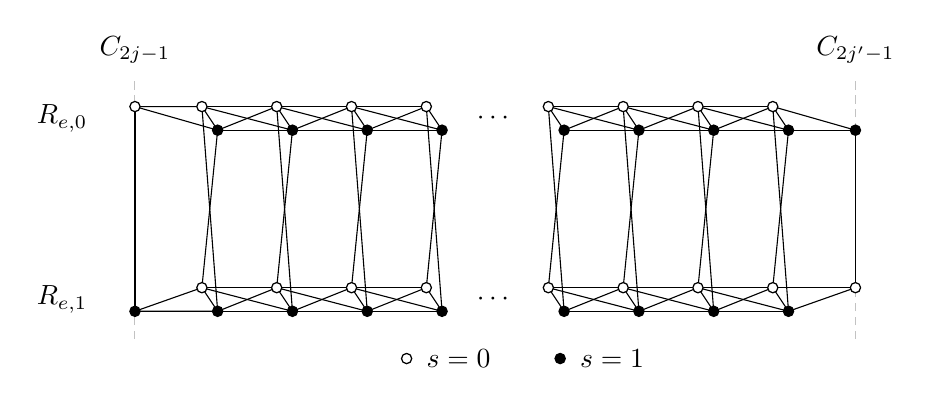
\begin{tikzpicture}[
  edge/.style={draw=black, line width=.4pt, line cap=round},
  guide/.style={draw=black!24, densely dashed, line width=.35pt},
  vertex/.style={circle, draw=black, line width=.45pt, minimum size=3.7pt, inner sep=0pt},
  side 0/.style={vertex, fill=white},
  side 1/.style={vertex, fill=black}
]
  \foreach \r/\y in {0/1.15,1/-1.15} {
    \foreach \c/\x in {1/.95,2/1.90,3/2.85,4/3.80,5/5.35,6/6.30,7/7.25,8/8.20} {
      \coordinate (v\r\c0) at ({\x-.10},{\y+.15});
      \coordinate (v\r\c1) at ({\x+.10},{\y-.15});
    }
  }
  \coordinate (v000) at (0,1.30);
  \coordinate (v101) at (0,-1.30);
  \coordinate (v091) at (9.15,1.00);
  \coordinate (v190) at (9.15,-1.00);

  \draw[guide] (0,-1.65) -- (0,1.65);
  \draw[guide] (9.15,-1.65) -- (9.15,1.65);
  \node[anchor=south] at (0,1.72) {$C_{2j-1}$};
  \node[anchor=south] at (9.15,1.72) {$C_{2j'-1}$};
  \node[anchor=east] at (-.48,1.15) {$R_{e,0}$};
  \node[anchor=east] at (-.48,-1.15) {$R_{e,1}$};

  \foreach \c in {1,2,3,4,5,6,7,8} {
    \foreach \r in {0,1} {
      \foreach \q in {0,1} \draw[edge] (v\r\c0) -- (v\q\c1);
    }
  }
  \draw[edge] (v000) -- (v101);
  \draw[edge] (v190) -- (v091);

  \foreach \r in {0,1} {
    \foreach \a/\b in {1/2,2/3,3/4,5/6,6/7,7/8} {
      \foreach \s in {0,1} {
        \foreach \t in {0,1} \draw[edge] (v\r\a\s) -- (v\r\b\t);
      }
    }
  }
  \foreach \s in {0,1} {
    \draw[edge] (v000) -- (v01\s);
    \draw[edge] (v101) -- (v11\s);
    \draw[edge] (v08\s) -- (v091);
    \draw[edge] (v18\s) -- (v190);
  }

  \foreach \r in {0,1} {
    \foreach \c in {1,2,3,4,5,6,7,8} {
      \node[side 0] at (v\r\c0) {};
      \node[side 1] at (v\r\c1) {};
    }
  }
  \node[side 0] at (v000) {};
  \node[side 1] at (v101) {};
  \node[side 1] at (v091) {};
  \node[side 0] at (v190) {};

  \node[fill=white, inner xsep=3pt] at (4.575,1.15) {$\cdots$};
  \node[fill=white, inner xsep=3pt] at (4.575,-1.15) {$\cdots$};

  \node[side 0] at (3.45,-1.90) {};
  \node[anchor=west] at (3.58,-1.90) {$s=0$};
  \node[side 1] at (5.40,-1.90) {};
  \node[anchor=west] at (5.53,-1.90) {$s=1$};
\end{tikzpicture}
\caption{The restriction of $G_F$ to the two rows reserved for $e=v_jv_{j'}$.}
\label{fig:edge-gadget}
\end{figure}

  \begin{claim}
\leavevmode
% lax begin Lax222097.ColumnGridExclusion
Graph $G$ excludes the $5 \times 5$ grid as an induced minor.
% lax end Lax222097.ColumnGridExclusion
  \end{claim}
\begin{claimproof}
\leavevmode
% lax begin Lax222097Proofs.columnGraph_excludes_inducedGrid
We first claim that every cycle of~$G$ contains two (adjacent) vertices in the same column but on different sides, i.e., of the form $(i,j,0)$ and $(i',j,1)$.
    Indeed, if one removes from $G$ all the edges with endpoints in the same column but on different sides, the resulting graph $G'$ is the disjoint union of $2m$ graphs $Q_{2n-1}$ obtained from two $(2n-1)$-vertex paths $P_{2n-1}$ by making the $j$th vertex of the first path adjacent to the $(j-1)$st and $(j+1)$st of the other path (when these vertices exist).
    In particular, consider a~\emph{leftmost} vertex $(\widehat{i},\widehat{j},s)$ (i.e., minimizing $\widehat{j}$) of a~cycle $C$ that does not contain a~pair $(i,j,0), (i',j,1)$. Its two neighbors on~$C$ must be $(\widehat{i},\widehat{j}+1,0)$ and $(\widehat{i},\widehat{j}+1,1)$; these two vertices form such a~pair.
    See~\cref{fig:cycle-forced-pair} for an illustration.

\begin{figure}[!ht]
\centering
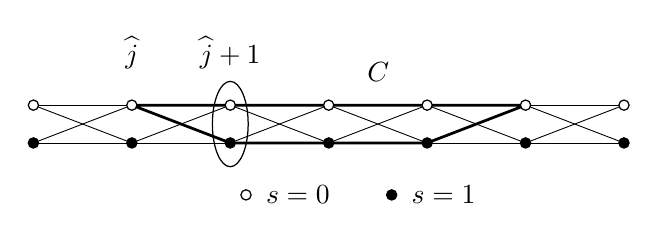
\begin{tikzpicture}[
  edge/.style={draw=black, line width=.32pt, line cap=round},
  cycle/.style={draw=black, line width=1pt, line cap=round, line join=round},
  vertex/.style={circle, draw=black, line width=.45pt,
    minimum size=3.7pt, inner sep=0pt},
  side 0/.style={vertex, fill=white},
  side 1/.style={vertex, fill=black},
  pair/.style={ellipse, draw=black, line width=.45pt,
    inner xsep=2.5pt, inner ysep=2pt}
]
  \foreach \c/\x in {0/0,1/1.25,2/2.50,3/3.75,4/5.00,5/6.25,6/7.50} {
    \coordinate (v\c0) at (\x,.24);
    \coordinate (v\c1) at (\x,-.24);
  }

  \foreach \a/\b in {0/1,1/2,2/3,3/4,4/5,5/6} {
    \foreach \s in {0,1} {
      \foreach \t in {0,1} \draw[edge] (v\a\s) -- (v\b\t);
    }
  }

  \draw[cycle] (v10) -- (v20) -- (v30) -- (v40) -- (v50) --
    (v41) -- (v31) -- (v21) -- cycle;

  \foreach \c in {0,1,2,3,4,5,6} {
    \node[side 0] (p\c0) at (v\c0) {};
    \node[side 1] (p\c1) at (v\c1) {};
  }

  \node[pair, fit=(p20)(p21)] {};
  \node[anchor=south] at (1.25,.58) {$\widehat{j}$};
  \node[anchor=south] at (2.50,.58) {$\widehat{j}+1$};
  \node[above] at (4.38,.42) {$C$};

  \node[side 0] at (2.70,-.90) {};
  \node[anchor=west] at (2.83,-.90) {$s=0$};
  \node[side 1] at (4.55,-.90) {};
  \node[anchor=west] at (4.68,-.90) {$s=1$};
\end{tikzpicture}
\caption{The leftmost-vertex argument in (a~connected component of) $G'$.}
\label{fig:cycle-forced-pair}
\end{figure}
    
\leavevmode
% lax begin Lax222097.AsteroidalCycles
Let $H$ be any graph with three vertex-disjoint and nonadjacent cycles $\Gamma_1, \Gamma_2, \Gamma_3$ such that there is a~path between any two cycles in the non-neighborhood of the third cycle.
\leavevmode
% lax begin Lax222097.CycleObstruction
Note that the $5 \times 5$ grid is such a~graph~$H$; see~\cref{fig:grid-three-cycles}.
% lax end Lax222097.CycleObstruction
% lax end Lax222097.AsteroidalCycles
    \begin{figure}[!ht]
\centering
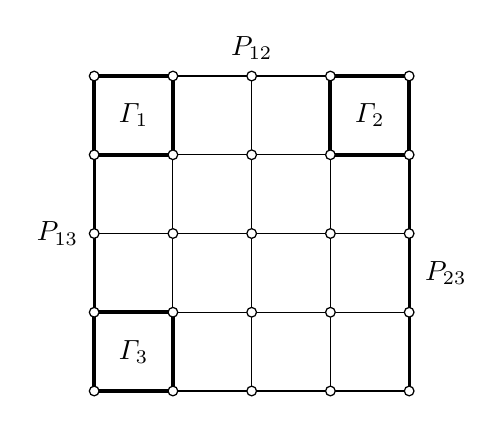
\begin{tikzpicture}[
  x=1cm,
  y=1cm,
  edge/.style={draw=black, line width=.35pt, line cap=round},
  cycle/.style={draw=black, line width=1.5pt, line cap=round, line join=round},
  connector/.style={draw=black, line width=1pt, line cap=round,
    preaction={draw=white, line width=1.7pt}},
  vertex/.style={circle, draw=black, fill=white, line width=.45pt,
    minimum size=3.5pt, inner sep=0pt}
]
  \foreach \x in {1,...,5} \draw[edge] (\x,1) -- (\x,5);
  \foreach \y in {1,...,5} \draw[edge] (1,\y) -- (5,\y);

  \draw[cycle] (1,4) -- (1,5) -- (2,5) -- (2,4) -- cycle;
  \draw[cycle] (4,4) -- (4,5) -- (5,5) -- (5,4) -- cycle;
  \draw[cycle] (1,1) -- (1,2) -- (2,2) -- (2,1) -- cycle;

  \draw[connector] (2,5) -- (3,5) -- (4,5);
  \draw[connector] (1,4) -- (1,3) -- (1,2);
  \draw[connector] (5,4) -- (5,3) -- (5,2) -- (5,1) -- (4,1) -- (3,1) -- (2,1);

  \foreach \x in {1,...,5} {
    \foreach \y in {1,...,5} \node[vertex] at (\x,\y) {};
  }

  \node at (1.5,4.5) {$\Gamma_1$};
  \node at (4.5,4.5) {$\Gamma_2$};
  \node at (1.5,1.5) {$\Gamma_3$};
  \node[anchor=south] at (3,5.08) {$P_{12}$};
  \node[anchor=east] at (.92,3) {$P_{13}$};
  \node[anchor=west] at (5.08,2.5) {$P_{23}$};
\end{tikzpicture}
\caption{Three appropriate cycles in the $5 \times 5$ grid.}
\label{fig:grid-three-cycles}
\end{figure}
    
\leavevmode
% lax begin Lax222097.CycleObstruction
We claim that no such graph $H$ is an induced minor of~$G$.
% lax end Lax222097.CycleObstruction
\leavevmode
% lax begin Lax222097Proofs.Obstruction.asteroidalCycles_obstruction
The subgraph of~$G$ induced by the union $U_a$ of the branch sets representing $V(\Gamma_a)$ (for any $a \in [3]$) has to contain a~cycle. 
    By the first paragraph, there are three column indices $j_1, j_2, j_3 \in [2n-1]$ such that $U_a$ contains a~pair of the form $(\cdot,j_a,0), (\cdot,j_a,1)$ for each $a \in [3]$.
    Without loss of generality, let us assume that $j_1 \leqslant j_2 \leqslant j_3$.
    Since the cycles $\Gamma_1, \Gamma_2, \Gamma_3$ are nonadjacent, we further have $j_1 < j_2 < j_3$.
    Finally, note that, for any $i,i' \in [2m]$, $N_G(\{(i,j_2,0), (i',j_2,1)\}) \supseteq C_{j_2}$ and that the removal of $C_{j_2}$ disconnects $C_{j_1}$ from $C_{j_3}$.
    This contradicts the assumption that there is a~path between $\Gamma_1$ and $\Gamma_3$ in the non-neighborhood of~$\Gamma_2$.
% lax end Lax222097Proofs.Obstruction.asteroidalCycles_obstruction
\claimqedhere
% lax end Lax222097Proofs.columnGraph_excludes_inducedGrid
  \end{claimproof}
\leavevmode
% lax begin Lax222097.GridExclusion
In particular, the induced subgraph $G_F$ of $G$ excludes the $5 \times 5$ grid as an induced minor.
% lax end Lax222097.GridExclusion
  We finish the proof by showing that computing the independence number of~$G_F$ would solve \textsc{Max Cut} for the arbitrary graph~$F$.
  
  \begin{claim}
\leavevmode
% lax begin Lax222097.IndependenceIdentity
$\alpha(G_F) = \maxcut(F) + 2 \sum\limits_{v_j v_{j'} \in E(F),~j<j'} j'-j$.
% lax end Lax222097.IndependenceIdentity
  \end{claim}
\begin{claimproof}
\leavevmode
% lax begin Lax222097Proofs.independence_eq_maxCut_offset
We first show that \[\alpha(G_F) \geqslant \maxcut(F) + 2 \sum\limits_{v_j v_{j'} \in E(F),~j<j'} j'-j.\]
    Let $(A_0,A_1)$ be a~bipartition of~$V(F)$ realizing the maximum cut.
    We identify $A_0$ (resp.~$A_1$) with the side $s=0$ (resp.~$s=1$).
    We build the independent set~$I$ as follows.

    For every $v_j \in A_0$ and every incident edge $e = v_jv_{j'} \in E(F)$, add to $I$ the unique vertex of $(R_{e,0} \cup R_{e,1}) \cap C_{2j-1} \cap S_0$.
    Note that this vertex is in $R_{e,0}$ if $j < j'$ and in $R_{e,1}$ if $j' < j$.
    Symmetrically, for every $v_j \in A_1$ and every incident edge $e = v_jv_{j'} \in E(F)$, add to $I$ the unique vertex of $(R_{e,0} \cup R_{e,1}) \cap C_{2j-1} \cap S_1$.

    At this stage, for every $e=v_jv_{j'} \in E(F)$ with, say, $j < j'$, $I$ intersects $R_{e,0} \cup R_{e,1}$ at exactly two vertices: one in $C_{2j-1}$ and one in $C_{2j'-1}$.
    Say that the former (the one in~$C_{2j-1}$) is in $R_{e,s}$, and that the latter is in $R_{e,s'}$, with $s, s' \in \{0,1\}$.
    We add the following vertices of $R_{e,0} \cup R_{e,1}$ to the independent set~$I$:
    \begin{itemize}
    \item for every $v_{j''} \in A_0$ with $j'' \in [j+1,j'-1]$, we add the vertex $(e^s,2j''-1,0)$;
    \item for every $v_{j''} \in A_1$ with $j'' \in [j+1,j'-1]$, we add the vertex $(e^s,2j''-1,1)$; 
    \item for every $j'' \in [j,j'-2]$, we add $(e^{1-s},2j'',0)$ to $I$;
    \item in addition, if $s=s'$, we add $(e^{1-s},2j'-2,0)$ to~$I$.
    \end{itemize}
    
    (Note that for the last two items, we could also have consistently picked the corresponding vertices in~$S_1$.
    In fact, we could have kept only a~single vertex at the intersection of a~row with a~column of even index, but we decided against that to simplify the description of~$G$.)
    This finishes the construction of~$I$.
    It is indeed an independent set as we observed the following rules:
    \begin{itemize}
    \item in every column, we only picked vertices from one side, and
    \item we never picked two vertices in consecutive columns of the same row.
    \end{itemize}
    
    We now determine the size of~$I$.
    For every $e=v_jv_{j'} \in E(F)$ with $j<j'$, $I \cap (R_{e,0} \cup R_{e,1})$ contains exactly one vertex in every column intersected by $R_{e,0} \cup R_{e,1}$ except possibly $C_{2j'-2}$, in which it contains at most one vertex.
    Thus \[|I \cap (R_{e,0} \cup R_{e,1})| \in \{2(j'-j),2(j'-j)+1\}.\]
    Furthermore, if $e$ is in the cut $(A_0,A_1)$, then $s=s'$ and $|I \cap (R_{e,0} \cup R_{e,1})| = 2(j'-j)+1$.
    See \cref{fig:alpha-lower-bound} for an illustration.
    Therefore, \[|I| = \maxcut(F) + 2 \sum\limits_{v_j v_{j'} \in E(F),~j<j'} j'-j,~~\text{as desired}.\]

\begin{figure}[!ht]
\centering
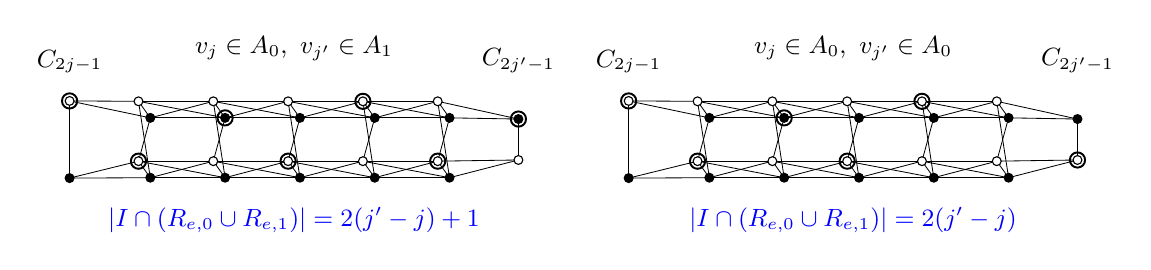
\begin{tikzpicture}[
  edge/.style={draw=black, line width=.3pt, line cap=round},
  vertex/.style={circle, draw=black, line width=.4pt, minimum size=3.2pt, inner sep=0pt},
  side 0/.style={vertex, fill=white},
  side 1/.style={vertex, fill=black},
  chosen/.style={circle, draw=black, line width=.7pt, minimum size=5.5pt, inner sep=0pt},
  panel label/.style={font=\small},
  count/.style={font=\small, text=blue}
]
  \foreach \p/\X/\a/\b in {c/0/0/1,n/7.10/0/0} {
    \begin{scope}[xshift={\X cm}]
    \foreach \r/\y in {0/.38,1/-.38} {
      \foreach \c/\x in {1/.95,2/1.90,3/2.85,4/3.80,5/4.75} {
        \coordinate (v\p\r\c0) at ({\x-.075},{\y+.105});
        \coordinate (v\p\r\c1) at ({\x+.075},{\y-.105});
      }
    }
    \coordinate (l\p0) at (0,.49);
    \coordinate (l\p1) at (0,-.49);
    \coordinate (r\p0) at (5.70,.26);
    \coordinate (r\p1) at (5.70,-.26);

    \foreach \c in {1,2,3,4,5} {
      \foreach \r in {0,1} {
        \foreach \q in {0,1} \draw[edge] (v\p\r\c0) -- (v\p\q\c1);
      }
    }
    \draw[edge] (l\p0) -- (l\p1);
    \draw[edge] (r\p0) -- (r\p1);
    \foreach \r in {0,1} {
      \foreach \a/\b in {1/2,2/3,3/4,4/5} {
        \foreach \s in {0,1} {
          \foreach \t in {0,1} \draw[edge] (v\p\r\a\s) -- (v\p\r\b\t);
        }
      }
      \foreach \s in {0,1} {
        \draw[edge] (l\p\r) -- (v\p\r1\s);
        \draw[edge] (v\p\r5\s) -- (r\p\r);
      }
    }

    \foreach \r in {0,1} {
      \foreach \c in {1,2,3,4,5} {
        \node[side 0] (p\p\r\c0) at (v\p\r\c0) {};
        \node[side 1] (p\p\r\c1) at (v\p\r\c1) {};
      }
    }
    \node[side 0] (pl\p0) at (l\p0) {};
    \node[side 1] (pl\p1) at (l\p1) {};
    \node[side 1] (pr\p0) at (r\p0) {};
    \node[side 0] (pr\p1) at (r\p1) {};

    \node[panel label] at (2.85,1.15) {$v_j\in A_{\a},\ v_{j'}\in A_{\b}$};
    \node[panel label, anchor=south] at (0,.72) {$C_{2j-1}$};
    \node[panel label, anchor=south] at (5.70,.72) {$C_{2j'-1}$};
    \end{scope}
  }

  \foreach \u in {plc0,pc110,pc021,pc130,pc040,pc150,prc0} \node[chosen, fit=(\u)] {};
  \foreach \u in {pln0,pn021,pn040,prn1,pn110,pn130} \node[chosen, fit=(\u)] {};

  \node[count] at (2.85,-1.02) {$|I\cap(R_{e,0}\cup R_{e,1})|=2(j'-j)+1$};
  \node[count] at (9.95,-1.02) {$|I\cap(R_{e,0}\cup R_{e,1})|=2(j'-j)$};

  %\node[side 0] at (5.00,-1.52) {};
  %\node[panel label, anchor=west] at (5.13,-1.52) {$s=0$};
  %\node[side 1] at (7.25,-1.52) {};
  %\node[panel label, anchor=west] at (7.38,-1.52) {$s=1$};
\end{tikzpicture}
\caption{Example of $I\cap(R_{e,0}\cup R_{e,1})$ (circled vertices) when $v_j$ and $v_{j'}$ are on opposite sides of the bipartition $(A_0,A_1)$ (left) and when they are on the same side (right).}
\label{fig:alpha-lower-bound}
\end{figure}

    We now show that \[\alpha(G_F) \leqslant \maxcut(F) + 2 \sum\limits_{v_j v_{j'} \in E(F),~j<j'} j'-j.\]
    We fix some independent set~$I$ of~$G_F$.
    In every column $C_{2j-1}$ of $v_j$, $I$ can only contain vertices from one side (because of the biclique between $S_0 \cap C_{2j-1}$ and $S_1 \cap C_{2j-1}$).
    The set $I$ thus defines a~partition $(A_0,A_1)$ of $V(F)$ where $v_j \in V(F)$ is in~$A_0$ if $I \cap C_{2j-1} \subseteq S_0$, and $v_j \in A_1$ if instead $I \cap C_{2j-1} \subseteq S_1$.
    For every $e=v_jv_{j'} \in E(F)$ with $j<j'$, we partition $R_{e,0} \cup R_{e,1}$ into $D_j, D_{j+1}, \ldots, D_{j'-1}, D_{j'}$, where
    \begin{itemize}
    \item $D_j := C_{2j-1} \cap (R_{e,0} \cup R_{e,1})$, and
    \item for every $j'' \in [j+1,j']$, $D_{j''} := (C_{2j''-2} \cup C_{2j''-1}) \cap (R_{e,0} \cup R_{e,1})$.
    \end{itemize}

    Observe that $I$ can contain at most one vertex in $D_j$, and at most two vertices in each $D_{j''}$ with $j'' \in [j+1,j']$.
    This implies that $|I \cap (R_{e,0} \cup R_{e,1})| \leqslant 1+2(j'-j)$; see~\cref{fig:alpha-upper-bound}.
    \begin{figure}[!ht]
\centering
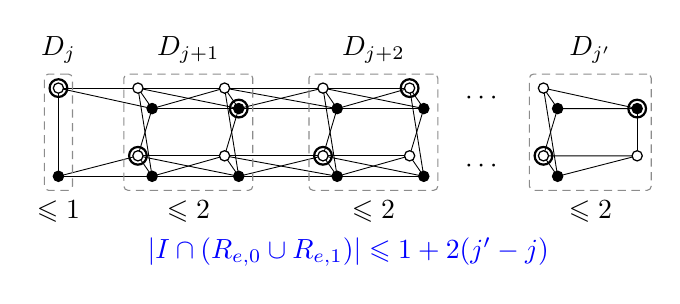
\begin{tikzpicture}[
  edge/.style={draw=black, line width=.32pt, line cap=round},
  vertex/.style={circle, draw=black, line width=.45pt, minimum size=3.7pt, inner sep=0pt},
  side 0/.style={vertex, fill=white},
  side 1/.style={vertex, fill=black},
  block/.style={draw=black!45, densely dashed, rounded corners=1.5pt, inner sep=3pt},
  chosen/.style={circle, draw=black, line width=.8pt, minimum size=6.4pt, inner sep=0pt}
]
  \foreach \r/\y in {0/.43,1/-.43} {
    \foreach \c/\x in {1/1.10,2/2.20,3/3.45,4/4.55,5/6.25} {
      \coordinate (v\r\c0) at ({\x-.09},{\y+.13});
      \coordinate (v\r\c1) at ({\x+.09},{\y-.13});
    }
  }
  \coordinate (l0) at (0,.56);
  \coordinate (l1) at (0,-.56);
  \coordinate (r0) at (7.35,.30);
  \coordinate (r1) at (7.35,-.30);

  \foreach \c in {1,2,3,4,5} {
    \foreach \r in {0,1} {
      \foreach \q in {0,1} \draw[edge] (v\r\c0) -- (v\q\c1);
    }
  }
  \draw[edge] (l0) -- (l1);
  \draw[edge] (r0) -- (r1);
  \foreach \r in {0,1} {
    \foreach \a/\b in {1/2,2/3,3/4} {
      \foreach \s in {0,1} {
        \foreach \t in {0,1} \draw[edge] (v\r\a\s) -- (v\r\b\t);
      }
    }
    \foreach \s in {0,1} {
      \draw[edge] (l\r) -- (v\r1\s);
      \draw[edge] (v\r5\s) -- (r\r);
    }
  }

  \foreach \r in {0,1} {
    \foreach \c in {1,2,3,4,5} {
      \node[side 0] (p\r\c0) at (v\r\c0) {};
      \node[side 1] (p\r\c1) at (v\r\c1) {};
    }
  }
  \node[side 0] (pl0) at (l0) {};
  \node[side 1] (pl1) at (l1) {};
  \node[side 1] (pr0) at (r0) {};
  \node[side 0] (pr1) at (r1) {};

  \node[block, fit=(pl0)(pl1)] (Dj) {};
  \node[block, fit=(p010)(p011)(p110)(p111)(p020)(p021)(p120)(p121)] (Djone) {};
  \node[block, fit=(p030)(p031)(p130)(p131)(p040)(p041)(p140)(p141)] (Djtwo) {};
  \node[block, fit=(p050)(p051)(p150)(p151)(pr0)(pr1)] (Djp) {};

  \node[anchor=south] at (Dj.north) {$D_j$};
  \node[anchor=south] at (Djone.north) {$D_{j+1}$};
  \node[anchor=south] at (Djtwo.north) {$D_{j+2}$};
  \node[anchor=south] at (Djp.north) {$D_{j'}$};
  \node[anchor=north] at (Dj.south) {$\leqslant 1$};
  \node[anchor=north] at (Djone.south) {$\leqslant 2$};
  \node[anchor=north] at (Djtwo.south) {$\leqslant 2$};
  \node[anchor=north] at (Djp.south) {$\leqslant 2$};

  \foreach \u in {pl0,p110,p021,p130,p040,p150,pr0} \node[chosen, fit=(\u)] {};
  \node[fill=white, inner xsep=3pt] at (5.40,.43) {$\cdots$};
  \node[fill=white, inner xsep=3pt] at (5.40,-.43) {$\cdots$};
  \node[anchor=north] at (3.68,-1.22)
    {\textcolor{blue}{$|I\cap(R_{e,0}\cup R_{e,1})|\leqslant 1+2(j'-j)$}};

  %\node[side 0] at (2.55,-1.95) {};
  %\node[anchor=west] at (2.70,-1.95) {$s=0$};
  %\node[side 1] at (4.70,-1.95) {};
  %\node[anchor=west] at (4.85,-1.95) {$s=1$};
\end{tikzpicture}
\caption{The partition $D_j, \ldots, D_{j'}$ and an upper bound on $|I\cap(R_{e,0}\cup R_{e,1})|$.}
\label{fig:alpha-upper-bound}
    \end{figure}
    Furthermore, if $v_j$ and $v_{j'}$ are on the same side of $(A_0,A_1)$, one can observe that $|I \cap (R_{e,0} \cup R_{e,1})| \leqslant 2(j'-j)$.

    We conclude that $|I| \leqslant \maxcut(F) + 2 \sum\limits_{v_j v_{j'} \in E(F),~j<j'} j'-j$.
\claimqedhere
% lax end Lax222097Proofs.independence_eq_maxCut_offset
  \end{claimproof}

  One can easily compute $2 \sum_{v_j v_{j'} \in E(F),~j<j'} j'-j$ in polynomial time.
  So we conclude that solving \smis on $G_F$ is as hard as solving \textsc{Max Cut} on~$F$.
\qedhere
% lax end Lax222097Proofs.independentSet_inducedGrid_hardness
\end{proof}

We obtain the following corollary by reducing from \textsc{Max Cut} on subcubic graphs.

\begin{repcorollary}{thm:eth}
  Unless the ETH fails, \mis requires $2^{\Omega(\sqrt{n})}$ time in $n$-vertex graphs excluding the $5 \times 5$ grid as an induced minor.
\end{repcorollary}

\begin{proof}
  By the Sparsification Lemma~\cite{sparsification}, under the ETH, $N$-variable \textsc{3-SAT-B} for some constant~$B$ (\textsc{3-SAT} where each variable appears at~most~$B$ times) has no $2^{o(N)}$-time algorithm.
  There is a~folklore linear reduction from \textsc{3-SAT-B} to~\textsc{Max 3-SAT-3} (\textsc{Max 3-SAT} where each variable appears at~most~three times).
  Composing the reductions in~\cite[Theorems 4.1 and 4.2]{Alimonti00} gives a~linear reduction from \textsc{Max E3-SAT-3} to \textsc{Max Cut} on subcubic graphs.
  We finally observe that applying the reduction in the proof of~\cref{thm:main} to subcubic \textsc{Max Cut} instances $F$ produces \smis instances with $n \leqslant 12|V(F)|^2$ vertices, so $n=\Oh(N^2)$.
\end{proof}

\paragraph*{AI disclosure.}
The reduction of~\cref{thm:main} was suggested by GPT-6 Pro after, embarrassingly, a~mere 23-minute think.
We simplified and improved the original complicated argument that the constructed instances exclude the $20 \times 20$ grid as an induced minor.
The write-up is entirely due to the authors.

\bibliography{main}

\end{document}
